\documentclass[]{book}
\usepackage{lmodern}
\usepackage{amssymb,amsmath}
\usepackage{ifxetex,ifluatex}
\usepackage{fixltx2e} % provides \textsubscript
\ifnum 0\ifxetex 1\fi\ifluatex 1\fi=0 % if pdftex
  \usepackage[T1]{fontenc}
  \usepackage[utf8]{inputenc}
\else % if luatex or xelatex
  \ifxetex
    \usepackage{mathspec}
  \else
    \usepackage{fontspec}
  \fi
  \defaultfontfeatures{Ligatures=TeX,Scale=MatchLowercase}
\fi
% use upquote if available, for straight quotes in verbatim environments
\IfFileExists{upquote.sty}{\usepackage{upquote}}{}
% use microtype if available
\IfFileExists{microtype.sty}{%
\usepackage{microtype}
\UseMicrotypeSet[protrusion]{basicmath} % disable protrusion for tt fonts
}{}
\usepackage[margin=1in]{geometry}
\usepackage{hyperref}
\hypersetup{unicode=true,
            pdftitle={Elementary Statistical Modeling for Applied Biostatistics},
            pdfauthor={Jeffrey A. Walker},
            pdfborder={0 0 0},
            breaklinks=true}
\urlstyle{same}  % don't use monospace font for urls
\usepackage{natbib}
\bibliographystyle{apalike}
\usepackage{color}
\usepackage{fancyvrb}
\newcommand{\VerbBar}{|}
\newcommand{\VERB}{\Verb[commandchars=\\\{\}]}
\DefineVerbatimEnvironment{Highlighting}{Verbatim}{commandchars=\\\{\}}
% Add ',fontsize=\small' for more characters per line
\usepackage{framed}
\definecolor{shadecolor}{RGB}{248,248,248}
\newenvironment{Shaded}{\begin{snugshade}}{\end{snugshade}}
\newcommand{\KeywordTok}[1]{\textcolor[rgb]{0.13,0.29,0.53}{\textbf{#1}}}
\newcommand{\DataTypeTok}[1]{\textcolor[rgb]{0.13,0.29,0.53}{#1}}
\newcommand{\DecValTok}[1]{\textcolor[rgb]{0.00,0.00,0.81}{#1}}
\newcommand{\BaseNTok}[1]{\textcolor[rgb]{0.00,0.00,0.81}{#1}}
\newcommand{\FloatTok}[1]{\textcolor[rgb]{0.00,0.00,0.81}{#1}}
\newcommand{\ConstantTok}[1]{\textcolor[rgb]{0.00,0.00,0.00}{#1}}
\newcommand{\CharTok}[1]{\textcolor[rgb]{0.31,0.60,0.02}{#1}}
\newcommand{\SpecialCharTok}[1]{\textcolor[rgb]{0.00,0.00,0.00}{#1}}
\newcommand{\StringTok}[1]{\textcolor[rgb]{0.31,0.60,0.02}{#1}}
\newcommand{\VerbatimStringTok}[1]{\textcolor[rgb]{0.31,0.60,0.02}{#1}}
\newcommand{\SpecialStringTok}[1]{\textcolor[rgb]{0.31,0.60,0.02}{#1}}
\newcommand{\ImportTok}[1]{#1}
\newcommand{\CommentTok}[1]{\textcolor[rgb]{0.56,0.35,0.01}{\textit{#1}}}
\newcommand{\DocumentationTok}[1]{\textcolor[rgb]{0.56,0.35,0.01}{\textbf{\textit{#1}}}}
\newcommand{\AnnotationTok}[1]{\textcolor[rgb]{0.56,0.35,0.01}{\textbf{\textit{#1}}}}
\newcommand{\CommentVarTok}[1]{\textcolor[rgb]{0.56,0.35,0.01}{\textbf{\textit{#1}}}}
\newcommand{\OtherTok}[1]{\textcolor[rgb]{0.56,0.35,0.01}{#1}}
\newcommand{\FunctionTok}[1]{\textcolor[rgb]{0.00,0.00,0.00}{#1}}
\newcommand{\VariableTok}[1]{\textcolor[rgb]{0.00,0.00,0.00}{#1}}
\newcommand{\ControlFlowTok}[1]{\textcolor[rgb]{0.13,0.29,0.53}{\textbf{#1}}}
\newcommand{\OperatorTok}[1]{\textcolor[rgb]{0.81,0.36,0.00}{\textbf{#1}}}
\newcommand{\BuiltInTok}[1]{#1}
\newcommand{\ExtensionTok}[1]{#1}
\newcommand{\PreprocessorTok}[1]{\textcolor[rgb]{0.56,0.35,0.01}{\textit{#1}}}
\newcommand{\AttributeTok}[1]{\textcolor[rgb]{0.77,0.63,0.00}{#1}}
\newcommand{\RegionMarkerTok}[1]{#1}
\newcommand{\InformationTok}[1]{\textcolor[rgb]{0.56,0.35,0.01}{\textbf{\textit{#1}}}}
\newcommand{\WarningTok}[1]{\textcolor[rgb]{0.56,0.35,0.01}{\textbf{\textit{#1}}}}
\newcommand{\AlertTok}[1]{\textcolor[rgb]{0.94,0.16,0.16}{#1}}
\newcommand{\ErrorTok}[1]{\textcolor[rgb]{0.64,0.00,0.00}{\textbf{#1}}}
\newcommand{\NormalTok}[1]{#1}
\usepackage{longtable,booktabs}
\usepackage{graphicx,grffile}
\makeatletter
\def\maxwidth{\ifdim\Gin@nat@width>\linewidth\linewidth\else\Gin@nat@width\fi}
\def\maxheight{\ifdim\Gin@nat@height>\textheight\textheight\else\Gin@nat@height\fi}
\makeatother
% Scale images if necessary, so that they will not overflow the page
% margins by default, and it is still possible to overwrite the defaults
% using explicit options in \includegraphics[width, height, ...]{}
\setkeys{Gin}{width=\maxwidth,height=\maxheight,keepaspectratio}
\IfFileExists{parskip.sty}{%
\usepackage{parskip}
}{% else
\setlength{\parindent}{0pt}
\setlength{\parskip}{6pt plus 2pt minus 1pt}
}
\setlength{\emergencystretch}{3em}  % prevent overfull lines
\providecommand{\tightlist}{%
  \setlength{\itemsep}{0pt}\setlength{\parskip}{0pt}}
\setcounter{secnumdepth}{5}
% Redefines (sub)paragraphs to behave more like sections
\ifx\paragraph\undefined\else
\let\oldparagraph\paragraph
\renewcommand{\paragraph}[1]{\oldparagraph{#1}\mbox{}}
\fi
\ifx\subparagraph\undefined\else
\let\oldsubparagraph\subparagraph
\renewcommand{\subparagraph}[1]{\oldsubparagraph{#1}\mbox{}}
\fi

%%% Use protect on footnotes to avoid problems with footnotes in titles
\let\rmarkdownfootnote\footnote%
\def\footnote{\protect\rmarkdownfootnote}

%%% Change title format to be more compact
\usepackage{titling}

% Create subtitle command for use in maketitle
\newcommand{\subtitle}[1]{
  \posttitle{
    \begin{center}\large#1\end{center}
    }
}

\setlength{\droptitle}{-2em}
  \title{Elementary Statistical Modeling for Applied Biostatistics}
  \pretitle{\vspace{\droptitle}\centering\huge}
  \posttitle{\par}
  \author{Jeffrey A. Walker}
  \preauthor{\centering\large\emph}
  \postauthor{\par}
  \predate{\centering\large\emph}
  \postdate{\par}
  \date{2018-08-28}

\usepackage{booktabs}
\usepackage{amsthm}
\makeatletter
\def\thm@space@setup{%
  \thm@preskip=8pt plus 2pt minus 4pt
  \thm@postskip=\thm@preskip
}
\makeatother

\usepackage{amsthm}
\newtheorem{theorem}{Theorem}[chapter]
\newtheorem{lemma}{Lemma}[chapter]
\theoremstyle{definition}
\newtheorem{definition}{Definition}[chapter]
\newtheorem{corollary}{Corollary}[chapter]
\newtheorem{proposition}{Proposition}[chapter]
\theoremstyle{definition}
\newtheorem{example}{Example}[chapter]
\theoremstyle{definition}
\newtheorem{exercise}{Exercise}[chapter]
\theoremstyle{remark}
\newtheorem*{remark}{Remark}
\newtheorem*{solution}{Solution}
\begin{document}
\maketitle

{
\setcounter{tocdepth}{1}
\tableofcontents
}
\chapter{Statistical Modeling}\label{statistical-modeling}

\emph{More cynically, one could also well ask ``Why has medicine not
adopted frequentist inference, even though everyone presents P-values
and hypothesis tests?'' My answer is: Because frequentist inference,
like Bayesian inference, is not taught. Instead everyone gets taught a
misleading pseudo-frequentism: a set of rituals and misinterpretations
caricaturing frequentist inference, leading to all kinds of
misunderstandings.} -- Sander Greenland

We use statistics to learn from data with uncertainty. Traditional
introductory textbooks in biostatistics implicitly or explicitly train
students and researchers to ``discover by p-value'' using hypothesis
tests (appendix xxx). Over the course of many chapters, the student is
trained to use something like a dichotomous key to choose the correct
``test'' for the data at hand, compute a test statistic for their data,
compute a \(p\)-value based on the test statistic, and compares the
\emph{p}-value to 0.05. Textbooks typically give very little guidance
about what can be concluded if \(p < 0.05\) or if \(p > 0.05\), but many
researchers conclude they have ``discovered'' something if \(p < 0.05\)
but found ``no effect'' if \(p > 0.05\).

Researchers learn almost nothing useful from a hypothesis test. If we
are investigating the effects of an increasingly acidified ocean on
coral growth, \(p=0.002\) may be evidence that pH affects growth, but,
from everything we know about pH and cell biology, it would be absurd to
conclude from any data that ocean acidification does not affect growth.
Instead, we want to know the magnitude of the effect and our uncertainty
in estimating this magnitude. We can use this magnitude and uncertainty
to make predictions about the future of coral reefs, under different
scenarios of ocean acidification. We can use the estimated effects and
uncertainty to model the consquences of the effects of acidification on
coral growth on fish production or carbon cycling.

The ``discovery by p-value'' strategy, or Null-Hypothesis Significance
Testing (NHST), has been criticized by statisticians for many, many
decades. Nevertheless, introductory biostatistics textbooks written by
both biologists and statisticians continue to organize textbooks around
a collection of hypothesis tests, with little emphasis on estimation and
uncertainty.

\section{Statistical modeling with linear
models}\label{statistical-modeling-with-linear-models}

This textbook is an introduction to the analysis of biological data
using a statistical modeling approach. As an introduction, the focus
will be linear models and extensions of the linear models including
linear mixed models and generalized linear models. Here, I refer to all
of these as ``linear models'' because all are a function of a linear
predictor. Linear models are the engine behind many hypothesis tests but
the emphasis in statistical modeling is estimation and uncertainty
instead of test statistics and \(p\)-values. A modeling view of
statistics is also more coherent than a dichotomous key strategy.

\begin{quote}
\textbf{Box}

linear mixed models are also known as multilevel models and hierarchical
models. Generalized linear models (GLMs) are frequently called
non-linear models. While it is true that the response (\(Y\)) is usually
a non-linear function of the \(X\) in a GLM, the expected values of
\(Y\) are a non-linear transformation of a linear predictor function
like that in equation \eqref{eq:lm}. A common phrase is that GLMs are
``linear in the parameters.''
\end{quote}

\begin{figure}
\centering
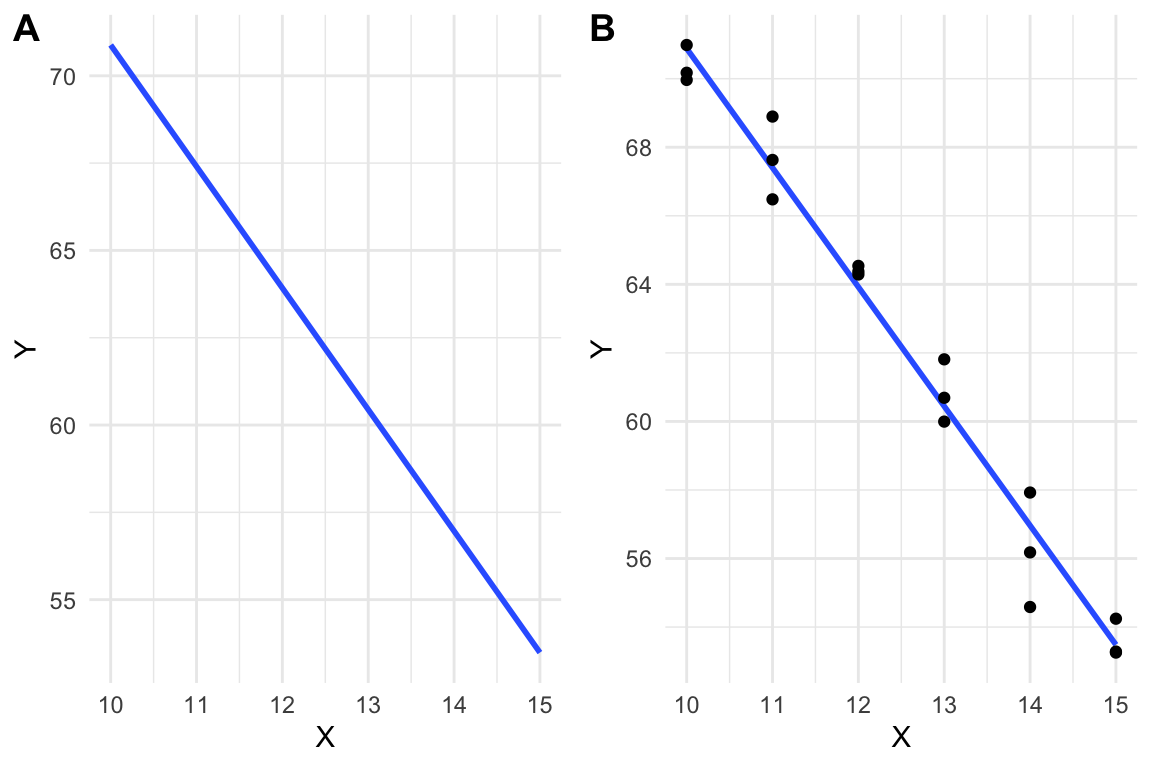
\includegraphics{Walker-elementary-statistical-odeling-draft_files/figure-latex/line-1.pdf}
\caption{\label{fig:line}A line vs.~a linear model. (A) the line \$y=-3.48X
+ 105.7 is drawn. (B) A linear model fit to the data. The model
coefficients are numerically equal to the slope and intercept of the
line in A.}
\end{figure}

All students are familiar with the idea of a linear model from learning
the equation of a line, which is

\begin{equation}
Y = mX + b
\label{eq:line}
\end{equation}

where \(m\) is the slope of the line and \(b\) is the \(Y\)-intercept.
It is useful to think of equation \eqref{eq:line} as a function that maps
values of \(X\) to values of \(Y\). Using this function, if we input
some value of \(X\), we always get the same value of Y as the output.

A linear model is a function, like that in equation \eqref{eq:line}, that
is fit to a set of data, often to model a process that generated the
data or something like the data. The line in Figure \ref{fig:line}A is
just that, a line, but the line in Figure \ref{fig:line}B is a model of
the data in Figure \ref{fig:line}B. The basic structure of a linear
model is

\begin{equation}
Y = \beta_0 + \beta_1 X + \varepsilon
\label{eq:lm}
\end{equation}

A linear model has two parts: the ``model''
(\(Y = \beta_0 + \beta_1 X\)) and the ``error'' (\(\varepsilon\)). The
model part looks like the equation for a line except that I've used
\(\beta_0\) for the intercept and \(\beta_1\) for the slope and I've put
the intercept term first. This re-labeling and re-arrangement make the
notation for a linear model more flexible for more complicated linear
models. For example
\(Y = \beta_0 + \beta_1 X_1 + \beta_2 X_2 + \varepsilon\) is a model
where \(Y\) is a function of two \(X\) variables.

As with the equation for a line, the model part of a linear model is a
function that maps a value of \(X\) to a specific value of \(Y\). This
mapped value is the \textbf{expected value} given a specific input value
of \(X\). The error part of a linear model is a random variable that
adds some random value to this expected value. Nothing about the model
part of a linear model can predict its value.

The inputs to a linear model (the \(X\) variables) have many names
including ``independent variables,'' ``predictor variables,'',
``explanatory variables,'' ``treatment variables,'' and ``covariates''.
The output of a linear model (the \(Y\) variable or variables if the
model is multivariate) is the ``dependent variable,'' ``response,'' or
``outcome.'' The \(\beta\) in the linear model are model
\textbf{parameters} There can be additional parameters in more
sophisticated models. The coefficients of the \(X\) in a linear model
(\(\beta_1\) in model \eqref{eq:lm}) are often called ``the effects'' (so
\(\beta_1\) is the effect of \(X_1\)).

Although a linear model is a model of a data-generating process, linear
models are not typically used to actually generate any data. Instead,
when we use a linear model to understand something about a real dataset,
we think of our data as one realization of a process that generates data
like ours. A linear model is a model of that process. That said, it is
incredibly useful to use linear models to create fake datasets for at
least two reasons: to probe our understanding of statistical modeling
generally and, more specifically, to check that a model actually creates
data like that in the real dataset that we are analyzing.

\subsection{Linear models are used for prediction, explanation, and
description}\label{linear-models-are-used-for-prediction-explanation-and-description}

Researchers typically use linear models to understand relationships
between one or more \(Y\) variables and one or more \(X\) variables.
These relationships include

\begin{enumerate}
\def\labelenumi{\arabic{enumi}.}
\item
  Descriptive modeling. Sometimes a researcher merely wants to describe
  the relationship between \(Y\) and a set of \(X\) variables, perhaps
  to discover patterns. For example, the arrival of a spring migrant
  bird (\(Y\)) as a function of sex (\(X_1\)) and age (\(X_2\)) might
  show that males and younger individuals arrive earlier. Importantly,
  if another \(X\) variable is added to the model (or one dropped), the
  coefficients, and therefore, the precise description, will change.
  That is, the interpretation of a coefficient as a descriptor is
  \emph{conditional} on the other covariates (\(X\) variables) in the
  model. In a descriptive model, there is no implication of causal
  effects and the goal is not prediction. Nevertheless, it is very hard
  for humans to discuss a descriptive model without using causal
  language, which probably means that it is hard for us to think of
  these models as \emph{mere description}. Like natural history,
  descriptive models are useful as patterns in want of an explanation,
  using more explicit causal models including experiments.
\item
  Predictive modeling. Predictive modeling is very common in applied
  research. For example, fisheries researchers might model the
  relationship between population density and habitat variables to
  predict which subset of ponds in a region are most suitable for brook
  trout (\emph{Salvelinus fontinalis}) reintroduction. The goal is to
  build a model with minimal prediction error, which is the error
  between predicted and actual values for a future sample. In predictive
  modeling, the \(X\) (``predictor'') variables are largely instrumental
  -- how these are related to \(Y\) is not a goal of the modeling,
  although sometimes an investigator may be interested in the relative
  importance among the \(X\) for predicting \(Y\) (for example,
  collecting the data may be time consuming, or expensive, or
  enviromentally destructive, so know which subset of \(X\) are most
  important for predicting \(Y\) is a useful strategy).
\item
  Explanatory (causal) modeling. Very often, researchers are explicitly
  interested in \emph{how} the \(X\) variables are causally related to
  \(Y\). The fisheries researchers that want to reintroduce trout may
  want to develop and manage a set of ponds to maintain healthy trout
  populations. This active management requires intervention to change
  habitat traits in a direction, and with a magnitude, to cause the
  desired response. This model is predictive -- a specific change in
  \(X\) predicts a specific response in \(Y\) -- because the
  coefficients of the model provide knowledge on how the system
  functions -- how changes in the inputs \emph{cause} change in the
  output. Causal interpretation of model coefficients requires a set of
  strong assumptions about the \(X\) variables in the model.
\end{enumerate}

Biologists are often not very explicit about which of these is the goal
of the modeling and use a combination of descriptive, predictive, and
causal language to describe and discuss results. By contrast,
researchers in economics and other social sciences, as well as
epidemiology and medicine more generally, are usually very explicit if
their model is descriptive, predictive, or causal.

\section{Model fitting}\label{model-fitting}

In order to use a linear model to describe, predict, or explain, we need
to fit a model to data. Instead of using an abtract model like that in
model \eqref{eq:lm}, I will introduce model fitting using data from Dryad
Data Repository.

\subsection{\texorpdfstring{A linear model with a single, continous
\(X\)}{A linear model with a single, continous X}}\label{a-linear-model-with-a-single-continous-x}

The data are from \citet{Dantzer_xxx}, who showed that North American
red squirrel (\emph{Tamiasciurus hudsonicus}) mothers from Yukon, Alaska
produce faster growing pups in years with increased squirrel density.
Remarkably, they even showed that perceived (but not actual) density
results in faster growing pups. To begin to investigate how pregnant
mothers control the future growth rate of pups, the researchers measured
the relationship between local squirrel density and the amount of fecal
cortisol metabolites from pregnant mothers. Cortisol is a hormone that
is secreted as part of stress response. The researchers were interested
in cortisol because it had previously been shownt that, in mammals,
blood cortisol levels in pregnant mothers have numerous effects on
offspring long past birth. If increased squirrel density causes
increased blood cortisol levels then we would expect to find a positive
relationship between \(Density\) and

\begin{figure}
\centering
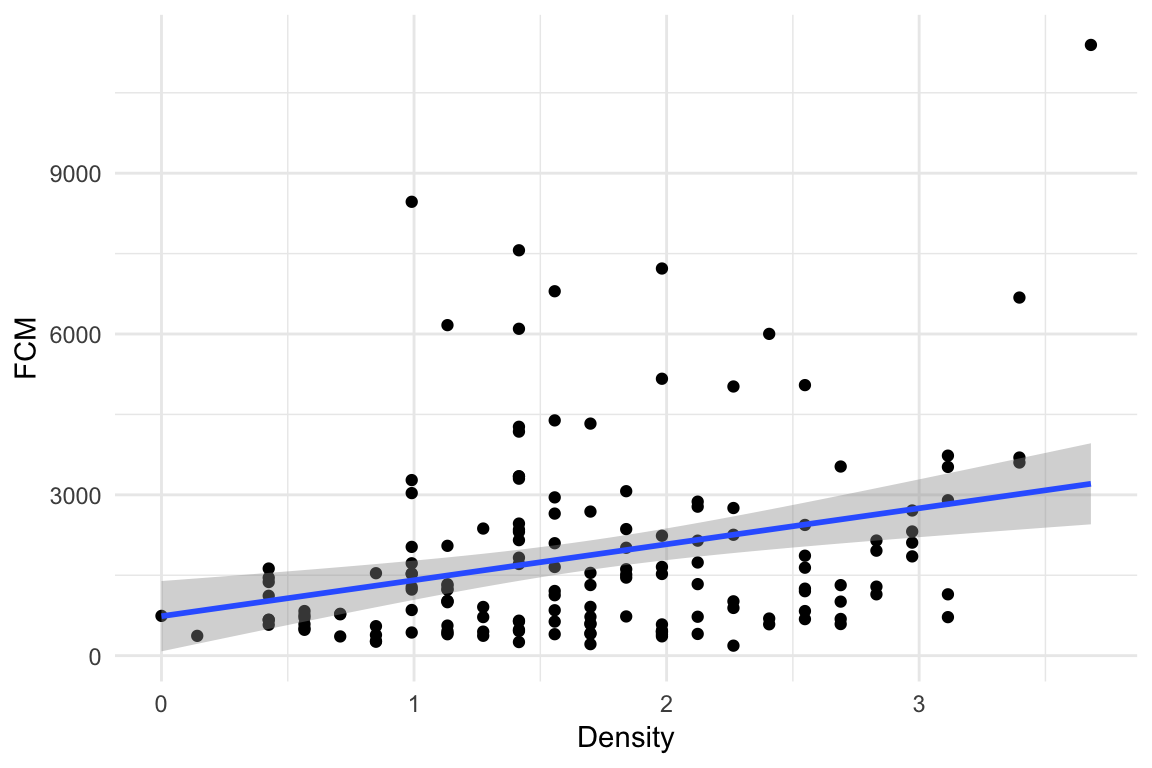
\includegraphics{Walker-elementary-statistical-odeling-draft_files/figure-latex/squirrel-1.pdf}
\caption{\label{fig:squirrel}A scatterplot of Fecal cortisol matabolites and
squirrel density.}
\end{figure}

Figure \ref{fig:squirrel} is a \textbf{scatterplot} of the data with the
amount of cortisol metabolites in the feces on the \(Y\) axis and local
squirrel density on the \(X\) axis. The line through the data is a
graphical representation of a linear model fit to the data and the gray
cloud around the line is a graphical representation of the uncertainty
in the model. The researchers wanted to model the ``effect'' of squirrel
density on the amount of cortisol metabolites in the feces of the
pregnant mothers. Graphically, this effect is the slope of the line in
Figure \ref{fig:squirrel}.

The model is

\begin{equation}
\textrm{E}[FCM|Density] = \beta_0 + \beta_1 Density
\label{eq:regression}
\end{equation}

In words, model \eqref{eq:regression} reads ``the expected value of
\(FCM\) conditional on density is beta-knot plus beta-one times
density''. An \textbf{expected value} is a long run average -- if we
were to sample lots and lots of red squirrel populations with
\(Density=x\) (where \(x\) is a specific value), we'd expect the average
\(FCM\) across these samples to be \(\beta_0 + \beta_1 x\).

In model \eqref{eq:regression}, there is a single \(X\) variable
(\(FCM\)). While the \(X\) variables are often called the ``dependent''
variables, in this model \(FCM\) does not ``depend'' on the independent
variable \(Density\) in any causal sense -- meaning if I were to
intervene and set \(Density\) to some value \(x\), I would expect
\(FCM\) to equal \(\beta_0 + \beta_1 x\). Rather, \(FCM\) only
``depends'' on \(Density\) in a probablistic sense -- if \(Density = x\)
then the most probable value of \(FCM\) is \(\beta_0 + \beta_1 x\). With
some strong assumptions model \eqref{eq:regression} can be turned into a
model of causal dependency, which is the focus of chapter xxx.

\(\beta_0\) and \(\beta_1\) are the \textbf{parameters} of model
\eqref{eq:regression}. Specifically \(\beta_0\) is the model
\textbf{intercept} and \(\beta_1\) is the modeled \textbf{effect} of
\(Density\). Again, the effect (\(\beta_1\)) has a probabilistic, and
not causal, interpretation. This interpretation is

\begin{equation}
\beta_1 = \textrm{E}[FCM|Density=x+1] - \textrm{E}[FCM|Density=x] 
\label{eq:beta1}
\end{equation}

Or, in words, ``beta-1 is the expected value of FCM when density equals
x + 1 minus the expected value of FCM when the density equals x.''
\(\beta_1\) is simply the difference in expected values given a one unit
difference in \(Density\).

\subsubsection{Using a linear model to estimate
effects}\label{using-a-linear-model-to-estimate-effects}

The goal of the statistical model here is to estimate \(\beta_1\) -- the
probabalistic effect of \(Density\) on \(FCM\). This estimate, and a
measure of the uncertainty of this estimate, are in the table of
coefficients of the fit model

\begin{verbatim}
##             Estimate Std. Error  t value     Pr(>|t|)
## (Intercept) 735.9604   331.9395 2.217152 0.0280776547
## Density     671.1380   178.8963 3.751549 0.0002483802
\end{verbatim}

where the entries in the column ``Estimate'' are estimates of the
parameters \(\beta_0\) and \(\beta_1\) in model \eqref{eq:regression}. The
entries in the column ``Std. Error'' are the standard errors (SE) of the
estimates, which are measures of the uncertainty of the estimates.

The parameter estimates in the table above are the coefficients of the
fitted model

\begin{equation}
FCM_i = b_0 + b_1 Density_i + e_i
\label{eq:fcmi}
\end{equation}

where the subscript \emph{i} refers to the \emph{i}th individual. The
coefficients \(b_0\) and \(b_1\) are the y-intercept and the slope of
the line in Figure \ref{fig:squirrel}. The coefficient for \(Density\)
(\(b_1\)) is 671.1, and (given the definition of the parameter
\(\beta_1\) in equation \eqref{eq:beta1}) we expect squirrel mothers with
a local density of 2 squirrels within a 150 m radius of her midden to
average 671.1 more units of FCM (ng of fecal cortical metabolites per
gram dry food) than mother squirrels with a local density of only 1
squirrel within a 150 m radius of her midden. Remember that this
coefficient is estimating a probabilistic parameter. Consequently, the
coefficient \(b_1\) is simply a descriptor of a pattern of relationship
between local density and fecal cortisol metabolites - no causal effect
is implied. With the strong assumptions explained in chapter xxx,
however, \(b_1\) can estimate a causal effect.

\subsubsection{Using a linear model for
prediction}\label{using-a-linear-model-for-prediction}

Model \eqref{eq:fcmi} gives the measured value of \emph{FCM} for each
squirrel. The equation includes the modeled part
(\(b_0 + b_1 Density_i\)) and the \textbf{residual} from the model
(\(e_i\)). The modeled part is the modeled or \textbf{predicted value},

\begin{equation}
\widehat{FCM} = b_0 + b_1 Density
\label{eq:fcmhat}
\end{equation}

where \(\widehat{FCM}\) is read as ``FCM hat''. Very often, we use the
model part (equation \eqref{eq:fcmhat}) to predict unknown or future
values given different modeled inputs (the \(X\)).

\subsection{\texorpdfstring{Linear models with categorical \(X\) are the
same as linear models with continuous
\(X\)}{Linear models with categorical X are the same as linear models with continuous X}}\label{linear-models-with-categorical-x-are-the-same-as-linear-models-with-continuous-x}

Singh et al. (xxx) studied the effect of parasite infection on the
production of recombinant offspring in several lines of fruit fly
\emph{Drosophila melanogaster}. Recombinant offspring are those with
allele combinations that do not occur in either parent.

\begin{figure}
\centering
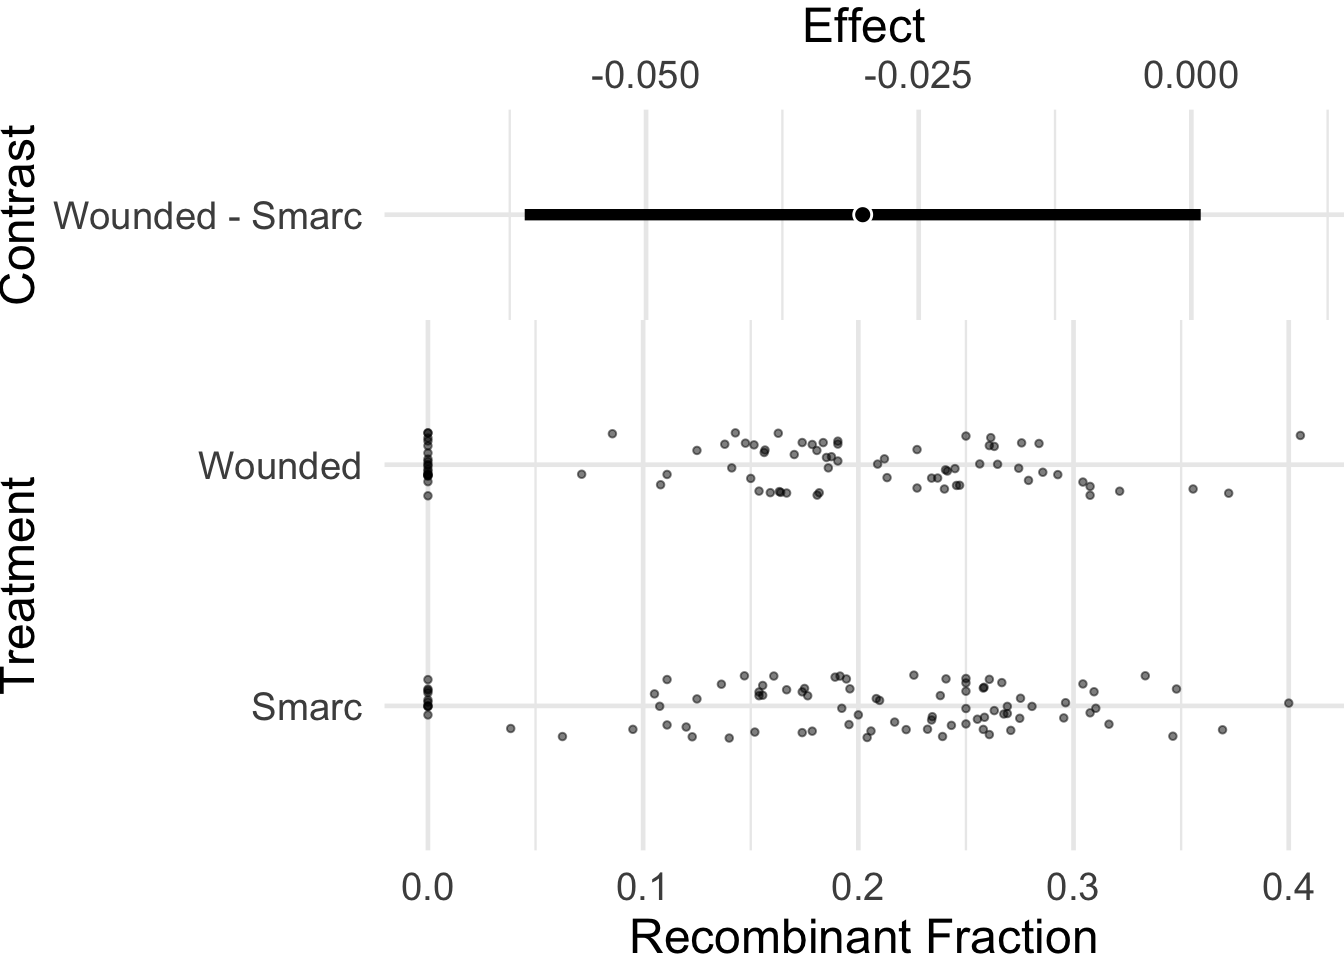
\includegraphics{Walker-elementary-statistical-odeling-draft_files/figure-latex/recombinantFlyPlot-1.pdf}
\caption{\label{fig:recombinantFlyPlot}Harrell plot of fly data. The bottom
part of the graph shows the data while the top part shows the effect
estimate and a measure of uncertainty. The specifics of the plot will be
explained in Chapter xxx. Briefly, the large black dots within the boxes
in the bottom part are the group mean recombinant frequencies. The black
dot in the top part of the plot is the difference in these group means
(the effect).}
\end{figure}

Figure \ref{fig:recombinantFlyPlot}, shows the results of one of the
experiments, specifically, the recombinant frequencies for each
replicate of the \textbf{treatment levels} ``Smarc'' (flies who were
parasitized by the bacteria \emph{Serratia marcescens}) and ``Wounded''
(flies who were given a sterile wound as a control). The mean of each
treatment level (or group) is shown with the large black dot within the
group's scatter of individual values, and the difference in the means is
shown in the top part with the black dot in the top part. The top plot
also shows a measure of the uncertainty in the estimate of this
difference (the thick black line).

The means of the two treatment levels (groups) are

\begin{verbatim}
##    Treatment      mean
## 1:     Smarc 0.1949128
## 2:   Wounded 0.1647802
\end{verbatim}

The difference between the means is 0.0301326. This is the estimate of
the effect of \emph{S. marcescens} parasitism on recombinant frequency.
In general, we wouldn't report these means or this difference in means
to this precision because the raw measures are not this precise but I do
it here because in order to compare this result to that of analzying the
data with a linear model.

The effect of \(Treatment\) can be modeled with the linear model

\begin{equation}
\textrm{E}[Recombinant\_fraction|Treatment] = \beta_0 + \beta_1 Treatment
\label{eq:categorical}
\end{equation}

The left side of this equation is read as ``the expected recombinant
fraction conditional on Treatment'' and can be thought of as ``the
expected recombinant fraction for a specific treatment level is equal
to\ldots{}''. Perhaps surprisingly, this is the same model as that used
for the squirrel fecal cortical metabolites, which is, more generally
\(\textrm{E}[Y|X] = \beta_0 + \beta_1 X\).

What are the estimates of \(\beta_0\) and \(\beta_1\)?

\begin{verbatim}
##                  Estimate Std. Error   t value     Pr(>|t|)
## (Intercept)    0.16478024 0.01129404 14.590016 8.719394e-32
## TreatmentSmarc 0.03013261 0.01570068  1.919191 5.663526e-02
\end{verbatim}

Compare the column ``Estimate'' with the group means and difference in
means computed above. The estimate of the intercept is the mean of the
Wounded group. The estimate of the \(Treatment\) coefficient is the
difference in means. That is,

\textbf{In a linear model with a categorical \(X\), the coefficients
(\(b_0\) and \(b_1\)) are a mean and a difference in means.}

The coefficients in the model with categorical \(X\) are also an
intercept and slope, and this is explored in the problems at the end of
the chapter, but it is not especially useful to think of them in this
way. In both kinds of models (categorical and continous \(X\)), we are
generally less interested in \(b_0\) and more interested in \(b_1\) --
the effect of \(X\).

For the recombinant fly experiment, the effect of bacteria infection is
0.03, or 3 additional recombinants per 100 offspring. The SE of this
effect (0.016) is our measure of uncertainty. The SE is used to compute
the 95\% confidence interval in the top part of figure
\ref{fig:recombinantFlyPlot}. The interval contains the range of effects
that are consistent with the data. This range includes values up to
about 6\% and down to about 0\%. Importantly, negative values (other
than very small ones) are not consistent with the data.

\subsection{\texorpdfstring{``Statistical model'' not ``regression
model''}{Statistical model not regression model}}\label{statistical-model-not-regression-model}

Statistical modeling terminology can be confusing. The \(X\) variables
in a statistical model may be quantitative (continuous or integers) or
categorical (names or qualitative amounts) or some mix of the two.
Linear models with all quantitative independent variables are often
called ``regression models.'' Linear models with all categorical
independent variables are often called ``ANOVA models''. Linear models
with a mix of quantitative and categorical variables are often called
``ANCOVA models'' if the focus is on one of the categorical \(X\) or
``regression models'' if there tend to be many independent variables.
These names reflect the history of the development of the different
kinds of linear models. I advocate using the term ``statistical model''
for general usage and ``linear model'' for more specific use, regardless
of the combination of variable types.

\section{Statistical modeling vs.~Null hypothesis
testing}\label{statistical-modeling-vs.null-hypothesis-testing}

Most biostatistics textbooks for biologists guide a student/researcher
toward the ``correct'' statistical test for experimental data. The
concept of a statistical test of inference is explored more in Appendix
xxx but for now, a typical textbook would probably steer a researcher
into analzying the recombinant fly data with a t-test of the difference
between means.

\begin{Shaded}
\begin{Highlighting}[]
\NormalTok{fly_t <-}\StringTok{ }\KeywordTok{t.test}\NormalTok{(Recombinant_fraction }\OperatorTok{~}\StringTok{ }\NormalTok{Treatment, }\DataTypeTok{data=}\NormalTok{sub_fly, }\DataTypeTok{var.equal=}\OtherTok{TRUE}\NormalTok{)}
\NormalTok{fly_t.p <-}\StringTok{ }\NormalTok{fly_t}\OperatorTok{$}\NormalTok{p.value}
\NormalTok{fly_t.t <-}\StringTok{ }\KeywordTok{abs}\NormalTok{(fly_t}\OperatorTok{$}\NormalTok{statistic)}
\end{Highlighting}
\end{Shaded}

The output of a \emph{t}-test is a test statistic (\emph{t}) and a
\emph{p}-value, which, roughly, is the probability of finding a test
statistic as large or larger than the observed test statistic if we were
to repeat the experiment many, many times using hypothetical data in
which there is no effect. This hypothetical data with no effect is the
\textbf{null hypothesis}.\footnote{The effect in the null hypotheses can
  be any pre-specified value. The nil null (zero effect) is the most
  common} A very small \emph{p} (say 0.01 or 0.0001) would be unlikely
if the null hypothesis were true, and, consequently, a very small
\emph{p} is evidence ``against the null'' (or evidence that a
low-probability event occurred, but we don't have additional evidence
for this so this conclusion is generally dismissed). Again, researchers
typically conclude that a difference is ``statistically significant'' if
\emph{p} is less than 0.05 and, consequently, the treatment has ``an
effect''.

The \emph{t}-statistic for the fly recombinant data is 1.9191906 and the
\emph{p}-value is 0.0566353, which means there is a 5.6\% probability of
finding \emph{t} \(\ge\) 1.9191906 if ``the null were true''. The
\emph{p}-value of 0.056 is a pretty small probability, and is close to
but not smaller than 0.05, and so is not ``statistically significant.''
How is this reported? If the researchers have an \emph{a priori}
hypothesis of an effect, they will often report a \emph{p}-value of
0.056 as ``marginally significant'' or worse ``trending toward
significant'' (why not trending ``away''?). But if the researchers have
an \emph{a priori} hypothesis of no effect, then they will often report
a \emph{p}-value of 0.056 as simply ``not significant'' or worse ``no
effect'' (see xxx why a \emph{p}-value is not evidence of no effect).

Most importantly, no part of null hypothesis testing is concerned with
estimating the effect size and our uncertainty in this estimate. Test
statistics and \emph{p}-values are not measures of effect size even
though each is a function of effect size. This is because each is also a
function of sample size and variation. A large \emph{t} and small
\emph{p} could result from a large effect, or a large sample, or small
variability. Null hypothesis testing encourages a focus on the trivia
(presence or absence of an effect) instead of the information that we
need to model a system. If we want to model the biological consquences
of an intervention, such as a drug, or of changing conditions, such as
ocean ocidification, or if we just want to model relationships within a
system, then we need measures of effect size and uncertainty from
statistical models.

A \emph{p}-value can is a useful, but limited tool, and a researcher can
use the statistical model to test specific hypotheses if desired. The
coefficients of the model are the simplest of these tests. Look at the
column ``Pr(\textgreater{}\textbar{}t\textbar{})'' in the table of
coefficients from the recombinant fly experiment above. This column
contains the probability of a \emph{t}-test for each coefficient. The
\emph{p} value for \(b_1\) (the Smarc treatment) is precisely the
\emph{p}-value for the \emph{t}-test of the means. This is because the
math behind a \emph{t}-test is a special case of the linear model in
model \eqref{eq:categorical}. And the math behind ANOVA is a special case
of the linear model. And the math behind regression is a special case of
the linear model. In other words, there is little reason to learn these
special cases as unrelated tests. There is no reason to teach (or learn)
the dichotomous key to the tests of inference.

\section{Multilevel models}\label{multilevel-models}

\section{Linear models versus non-linear
models}\label{linear-models-versus-non-linear-models}

In this text, I use ``linear model'' for any model that is linear in the
parameters, which means that the different components of the model are
added together. Or, using the language of matrix algebra, the predictor
is a simple dot product of the model matrix and the coefficients. For
example, a cubic polynomial model

\begin{equation}
Y = \beta_0 + \beta_1 X + \beta_2 X^2 + \beta_3 X^3 + \varepsilon
\end{equation}

is a linear model, even though the function is non-linear, because the
different components are added (or, using matrix algebra, the predictor
is \(\mathbf{X}\boldsymbol{\beta}\)).

A generalized linear model (GLM) has the form \(g(\mu_i) = \eta_i\)
where \(\eta\) (the greek letter eta) is the linear predictor, which is
linear in the parameters.

\begin{equation}
\eta = \mathbf{X}\boldsymbol{\beta} 
\end{equation}

Many sources do not consider a GLM to be a ``linear model'' but an
``extension'' of a linear model. Regardless, a GLM is linear in the
parameters and in this textbook, I include GLMs under the ``linear
model'' umbrella.

Non-linear models, in conrast to a GLM or classical linear model, are
not linear in the parameters (the predictor is not a simple dot product
of the model matrix and a vector of parameters). For example, the
Michaelis-Menten model is a nonlinear model

\begin{equation}
Y = \frac{\beta_1 X}{\beta_2 + X} + \varepsilon
\end{equation}

\chapter{Variability and Uncertainty (Standard Deviations and Standard
Errors)}\label{variability-and-uncertainty-standard-deviations-and-standard-errors}

\textbf{Uncertainty} is the stuff of science. A major goal of statistics
is measuring uncertainty. What do we mean by uncertainty? Uncertainty is
the error in estimating a parameter, such as the mean of a sample, or
the difference in means between two experimental treatments, or the
predicted response given a certain change in conditions. Uncertainty is
measured with a \textbf{variance} or its square root, which is a
\textbf{standard deviation}. The standard deviation of a statistic is
also (and more commonly) called a \textbf{standard error}.

Uncertainty emerges because of variability. In any introductory
statistics class, students are introduced to two measures of
variability, the ``standard deviation'' and the ``standard error.''
These terms are absolutely fundamental to statistics -- they are the
start of everything else. Yet, many biology professors confuse these
terms and certainly, introductory students do too.

When a research biologist uses the term ``standard deviation,'' they are
probably referring to the sample standard deviation which is a measure
of the variability of a sample. When a research biologist uses the term
``standard error,'' they are probably referring to the standard error of
a mean, but it could be the standard error of another statistics, such
as a regression slope. An important point to remember and understand is
that all standard errors \emph{are} standard deviations. This will make
more sense soon.

\section{The sample standard deviation vs.~the standard error of the
mean}\label{the-sample-standard-deviation-vs.the-standard-error-of-the-mean}

\subsection{Sample standard deviation}\label{sample-standard-deviation}

The sample standard deviation is a measure of the variability of a
sample. For example, were we to look at a histological section of
skeletal muscle we would see that the diameter of the fibers (the muscle
cells) is variable. We could use imaging software to measure the
diameter of a sample of 100 cells and get a \textbf{distribution} like
this

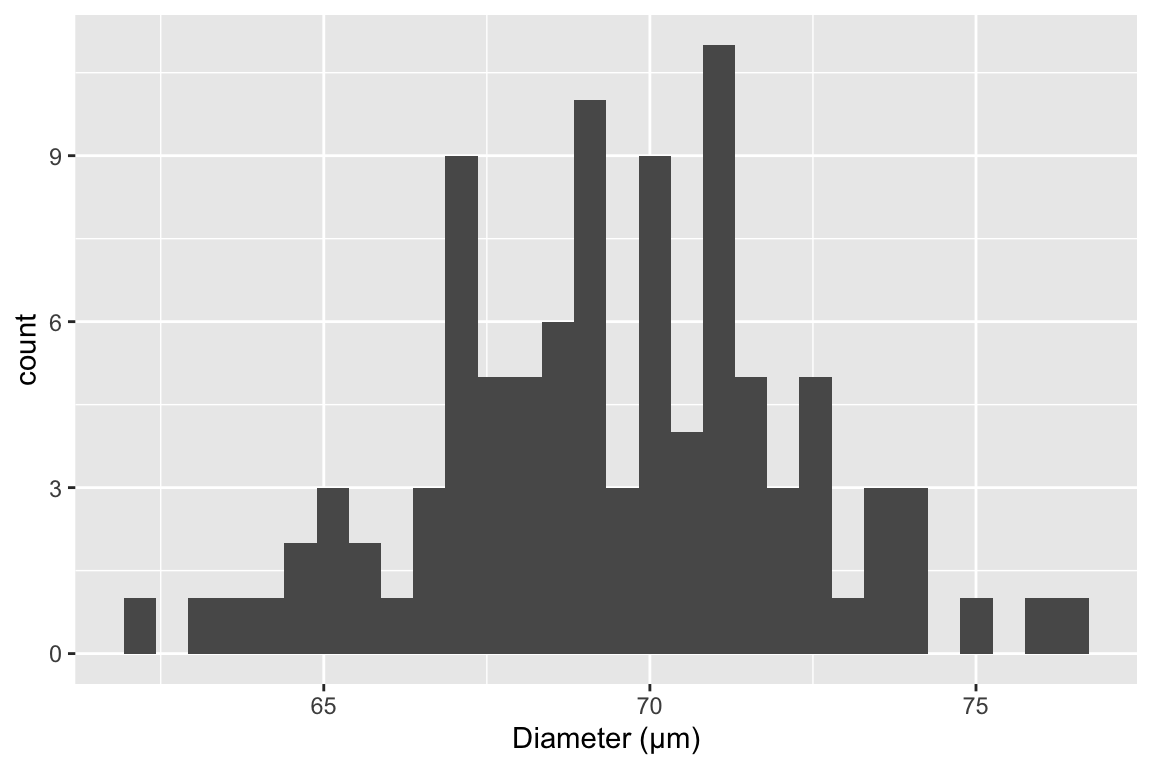
\includegraphics{Walker-elementary-statistical-odeling-draft_files/figure-latex/histogram-1.pdf}

The mean of this sample is 69.4 and the standard deviation is 2.8. The
standard deviation is the square root of the variance, and so computed
by

\begin{equation}
s_y = \sqrt{\frac{\sum_{i=1}^n{(y_i - \overline{y})^2}}{n-1}}
\label{eq:variance}
\end{equation}

Memorize this equation. To understand the logic of this measure of
variability, note that \(y_i - \overline{y}\) is the deviation of the
\(i\)th value from the sample mean, so the numerator is the sum of
squared deviations. The numerator is a sum over \(n\) items and the
denominator is \(n-1\) so the variance is (almost!) an averaged squared
deviation. More variable samples will have bigger deviations and,
therefore, bigger average squared deviations. Since the standard
deviation is the square root of the variance, a standard deviation is
the square root of the average squared deviation, it can be thought of
as a (not ``the'') measure of an average deviation.

Notes on the variance and standard deviation 1. Variances are additive
but standard deviations are not. This means that the variance of the sum
of two independent (uncorrelated) random variables is simply the sum of
the variances of each of the variables. This is important for many
statistical analyses. 2. The units of variance are the square of the
original units, which is awkward for interpretation. The units of a
standard deviation is the same as that of the original variable, and so
is much easier to interpet. 3. For variables that are approximately
normally distributed, we can map the standard deviation to the quantiles
of the distribution. For example, 68\% of the values are within one
standard deviation of the mean, 95\% of the values are within two
standard deviations, and 99\% of the values are within three standard
deviations.

\subsection{Standard error of the
mean}\label{standard-error-of-the-mean}

A standard error of a statistic is a measure of the precision of the
statistic. The standard error of the mean is a measure of the precision
of the mean. The smaller the value the more precise the estimate. The
standard error of the mean (SEM) is computed as

\begin{equation}
SEM = \frac{s_y}{sqrt{n}}
\label{eq:se}
\end{equation}

The SEM is often denoted \(s_{\bar{y}}\) to indicate that it is a
standard deviation of the mean (\(\bar{y}\). In what sense is a standard
error a measure of variability? This is kinda weird. If we sample 100
cells cells in the slide one time and compute the mean diameter, how can
the mean have a standard deviation? There is only one value! To
understand how the SEM is a standard deviation, imagine resampling 100
cells and recomputing a mean an infinite number of times and each time,
you write down the newly computed mean. The standard error of the mean
is the standard deviation of this infinitely long column of means.

Notes on standard errors 1. The SEM is only one kind of standard error.
A standard deviation can be computed for any statistics -- these are all
standard errors. For some statistics, such as the mean, the standard
error can be computed directly using an equation, such as that for the
SEM (equation @ref\{eq:se\}). For other statistics, a computer intensive
method such as the \textbf{bootstrap} is necessary to compute a standard
error. We will return to the bootstrap shortly. 2. The units of a
standard error are the units of the measured variable. 3. A standard
error is proportional to sample variability (the sample standard
deviation, \(s_y\)) and inversely proportional to sample size (\(n\)).
Sample variability is a function of both natural variation (there really
is variation in diameter among fibers in the quadriceps muscle) and
measurement error (imaging software with higher resolution can measure a
diameter with less error). Since the SEM is a measure of the precision
of estimating a mean, this means this precision will increase (or the
SEM will decrease) if 1) an investigator uses methods that reduce
measurement error and 2) an investigator computes the mean from a larger
sample. 4. This last point (the SEM decreases with sample size) seems
obvious when looking at equation @ref\{eq:se\}, since \(n\) is in the
denominator. Of course \(n\) is also in the denominator of equation
@ref\{eq:variance\} for the sample standard deviation (eq) but the
standard deviation does not decrease as sample size increases. First
this would make any sense -- variability is variability. A sample of
10,000 cell diameters should be no more variable than a sample of 100
cell diameters. Second, this should also be obvious from equation
@ref\{eq:variance\}. The standard deviation is the square root of an
average and averages don't increase with the number of things measured
since both the the numerator (a sum) and denominator increase with
\(n\).

\section{Using Google Sheets to generate fake data to explore
uncertainty}\label{using-google-sheets-to-generate-fake-data-to-explore-uncertainty}

In statistics we are interested in estimated parameters of a
\textbf{population} using measures from a \textbf{sample}. The goal in
this section is to use Google Sheets (or Microsoft Excel) to use fake
data to discover the behavior of sampling and to gain some intuition
about uncertainty using standard errors.

\subsection{Steps}\label{steps}

\begin{enumerate}
\def\labelenumi{\arabic{enumi}.}
\tightlist
\item
  Open Google Sheets
\item
  In cell A1 type ``Mu''. Mu is the greek letter \(\mu\) and is very
  common notation for the poplation value (the TRUE value!) of the mean
  of some hypothetical measure. In cell B1, insert some number as the
  value of \(\mu\). Any number! It can be negative or positive.
\item
  In cell A2 type ``Sigma''. Sigma is the greek letter \(\sigma\).
  \(\sigma^2\) is very common (universal!) notation for the population
  (TRUE) variance of some measure or parameter. Notice that the true
  (population) values of the mean and variance are greek letters. This
  is pretty standard in statistics. In cell B2, insert some positive
  number (standard deviations are the positive square roots of the
  variance).
\item
  In cell A8 type the number 1
\item
  In cell A9 insert the equation ``=A8 + 1''. What is this equation
  doing? It is adding the number 1 to to the value in the cell above, so
  the resulting value should be 2.
\item
  In Cell B8, insert the equation ``=normsinv(rand())*\$B\$2 + \$B\$1``.
  The first part of the equation creates a random normal variable with
  mean 0 and standard deviation 1. multiplication and addition transform
  this to a random normal variable with mean \(\mu\) and standard
  deviation \(\sigma\) (the values you set in cells B1 and B2).
\item
  copy cell B8 and paste into cell B9. Now Higlight cells A9:B9 and copy
  the equations down to row 107. You now have 100 random variables
  sampled from a infinite population with mean \(\mu\) and standard
  deviation \(\sigma\).
\item
  In cell A4 write ``mean 10''. In cell B4 insert the equation
  ``=average(B8:B17)''. The resulting value is the \textbf{sample mean}
  of the first 10 random variables you created. Is the mean close to
  \(\mu\)?
\item
  In cell A5 write ``sd 10''. In cell B5 insert the equation
  ``stdev(B8:B17)''. The result is the \textbf{sample standard
  deviation} of the first 10 random variables. Is this close to
  \(\sigma\)?
\item
  In cell A6 write ``mean 100''. In cell B6 insert the equation
  ``=average(B8:B107)''. The resulting value is the \textbf{sample mean}
  of the all 100 random variables you created. Is this mean closer to
  \(\mu\) than mean 10?
\item
  In cell A7 write ``sd 100''. In cell B7 insert the equation
  ``=stdev(B8:B107)''. The resulting value is the \textbf{sample
  standard deviation} of the all 100 random variables you created. Is
  this SD closer to \(\sigma\) than sd 10?
\end{enumerate}

The sample standard deviation is a measure of the variability of the
sample. The more spread out the sample (the further each value is from
the mean), the bigger the sample standard deviation. The sample standard
deviation is most often simply known as ``The'' standard deviation,
which is a bit misleading since there are many kinds of standard
deviations!

Remember that your computed mean and standard deviations are estimates
computed from a sample. They are estimates of the true values \(\mu\)
and \(\sigma\). Explore the behavior of the sample mean and standard
deviation by re-calculating the spreadsheet. In Excel, a spreadsheet is
re-calculated by simultaneously pressing the command and equal key. In
Google, command-R recalculates but is painfully slow. Instead, if using
Google Sheets, just type the number 1 into a blank cell, and the sheet
recalculates quickly. Do it again. And again.

Each time you re-calculate, a new set of random numbers are generated
and the new means and standard deviations are computed. Compare mean 10
and mean 100 each re-calculation. Notice that these estimates are
variable. They change with each re-calculation. How variable is mean 10
compared to mean 100? The variability of the estimate of the mean is a
measure of \textbf{uncertainty} in the estimate. Are we more uncertain
with mean 10 or with mean 100? This variability is measured by a
standard deviation. This \textbf{standard deviation of the mean} is also
called the \textbf{standard error of the mean}. Many researchers are
loose with terms and use ``The'' standard error to mean the standard
error of the mean, even though there are many kinds of standard errors.
In general, ``standard error''" is abbreviated as ``SE.'' Sometimes
``standard error of the mean'' is specifically abbreviated to ``SEM.''

The standard error of the mean is a measure of the precision in
estimating the mean. The smaller the value the more precise the
estimate. The standard error of the mean \emph{is} a standard deviation
of the mean. This is kinda weird. If we sample a population one time and
compute a mean, how can the mean have a standard deviation? There is
only one value! And we compute this value using the sample standard
deviation: \(SEM = \frac{SD}{\sqrt{N}}\). To understand how the SEM is a
standard deviation, Imagine recalculating the spread sheet an infinite
number of times and each time, you write down the newly computed mean.
The standard error of the mean is the standard deviation of this
infinitely long column of means.

\section{Using R to generate fake data to explore
uncertainty}\label{using-r-to-generate-fake-data-to-explore-uncertainty}

due by the beginning of our next class

note that I use ``standard deviation'' to refer to the sample standard
deviation and ``standard error'' to refer to the standard error of the
mean (again, we can compute standard errors as a standard deviation of
any kind of estimate)

\subsection{part I}\label{part-i}

In the exercise above, you used Google Sheets to generate \(p\) columns
of fake data. Each column had \(n\) elements, so the matrix of fake data
was \(n \times m\) (it is standard in most fields to specify a matrix as
rows by columns). This is \emph{much} easier to do in R and how much
grows exponentially as the size of the matrix grows.

To start, we just generate a \(n \times m\) matrix of normal random
numbers.

\begin{Shaded}
\begin{Highlighting}[]
\CommentTok{# R script to gain some intuition about standard deviation (sd) and standard error (se)}
\CommentTok{# you will probably need to install ggplot2 using library(ggplot2) }
\NormalTok{n <-}\StringTok{ }\DecValTok{6} \CommentTok{# sample size}
\NormalTok{p <-}\StringTok{ }\DecValTok{100} \CommentTok{# number of columns of fake data to generate}
\NormalTok{fake_data <-}\StringTok{ }\KeywordTok{matrix}\NormalTok{(}\KeywordTok{rnorm}\NormalTok{(n}\OperatorTok{*}\NormalTok{p, }\DataTypeTok{mean=}\DecValTok{0}\NormalTok{, }\DataTypeTok{sd=}\DecValTok{1}\NormalTok{), }\DataTypeTok{nrow=}\NormalTok{n, }\DataTypeTok{ncol=}\NormalTok{p) }\CommentTok{# create a matrix}
\end{Highlighting}
\end{Shaded}

the 3rd line is the cool thing about R. In one line I'm creating a
dataset with \(n\) rows and \(p\) columns. Each column is a sample of
the standard normal distribution which by definition has mean zero and
standard deviation of 1. But, and this is important, any sample from
this distribution will not have exactly mean zero and standard deviation
of 1, because it's a sample, the mean and standard deviation will have
some small errror from the truth. The line has two parts to it: first
I'm using the function ``rnorm'' (for random normal) to create a vector
of n*m random, normal deviates (draws from the random normal
distribution) and then I'm organizing these into a matrix (using the
function ``matrix'')

To compute the vector of means, standard deviations, and standard errors
for each column of \texttt{fake\_data}, use the \texttt{apply()}
function.

\begin{Shaded}
\begin{Highlighting}[]
\NormalTok{means <-}\StringTok{ }\KeywordTok{apply}\NormalTok{(fake_data,}\DecValTok{2}\NormalTok{,mean) }\CommentTok{# the apply function is super useful}
\NormalTok{sds <-}\StringTok{ }\KeywordTok{apply}\NormalTok{(fake_data,}\DecValTok{2}\NormalTok{,sd)}
\NormalTok{sems <-}\StringTok{ }\NormalTok{sds}\OperatorTok{/}\KeywordTok{sqrt}\NormalTok{(n)}
\end{Highlighting}
\end{Shaded}

\texttt{apply()} is a workhorse in many R scripts. Learn it. Know it.
Live it.

The SEM is the standard deviation of the mean, so let's see if the
standard deviation of the means is close to the true standard error. We
sampled from a normal distribution with SD=1 so the true standard is

\begin{Shaded}
\begin{Highlighting}[]
\DecValTok{1}\OperatorTok{/}\KeywordTok{sqrt}\NormalTok{(n)}
\end{Highlighting}
\end{Shaded}

\begin{verbatim}
## [1] 0.4082483
\end{verbatim}

and the standard deviation of the \(p\) means is

\begin{Shaded}
\begin{Highlighting}[]
\KeywordTok{sd}\NormalTok{(means)}
\end{Highlighting}
\end{Shaded}

\begin{verbatim}
## [1] 0.3731974
\end{verbatim}

Questions

\begin{enumerate}
\def\labelenumi{\arabic{enumi}.}
\tightlist
\item
  how close is \texttt{sd(means)} to the true SE?
\item
  change p above to 1000. Now how close is sd(means) to the true SE?
\item
  change p above to 10,000. Now how close is sd(means) to the true SE?
\end{enumerate}

\subsection{part II - means}\label{part-ii---means}

This is a visualization of the spread, or variability, of the sampled
means

\begin{Shaded}
\begin{Highlighting}[]
\KeywordTok{qplot}\NormalTok{(means)}
\end{Highlighting}
\end{Shaded}

\begin{verbatim}
## `stat_bin()` using `bins = 30`. Pick better value with `binwidth`.
\end{verbatim}

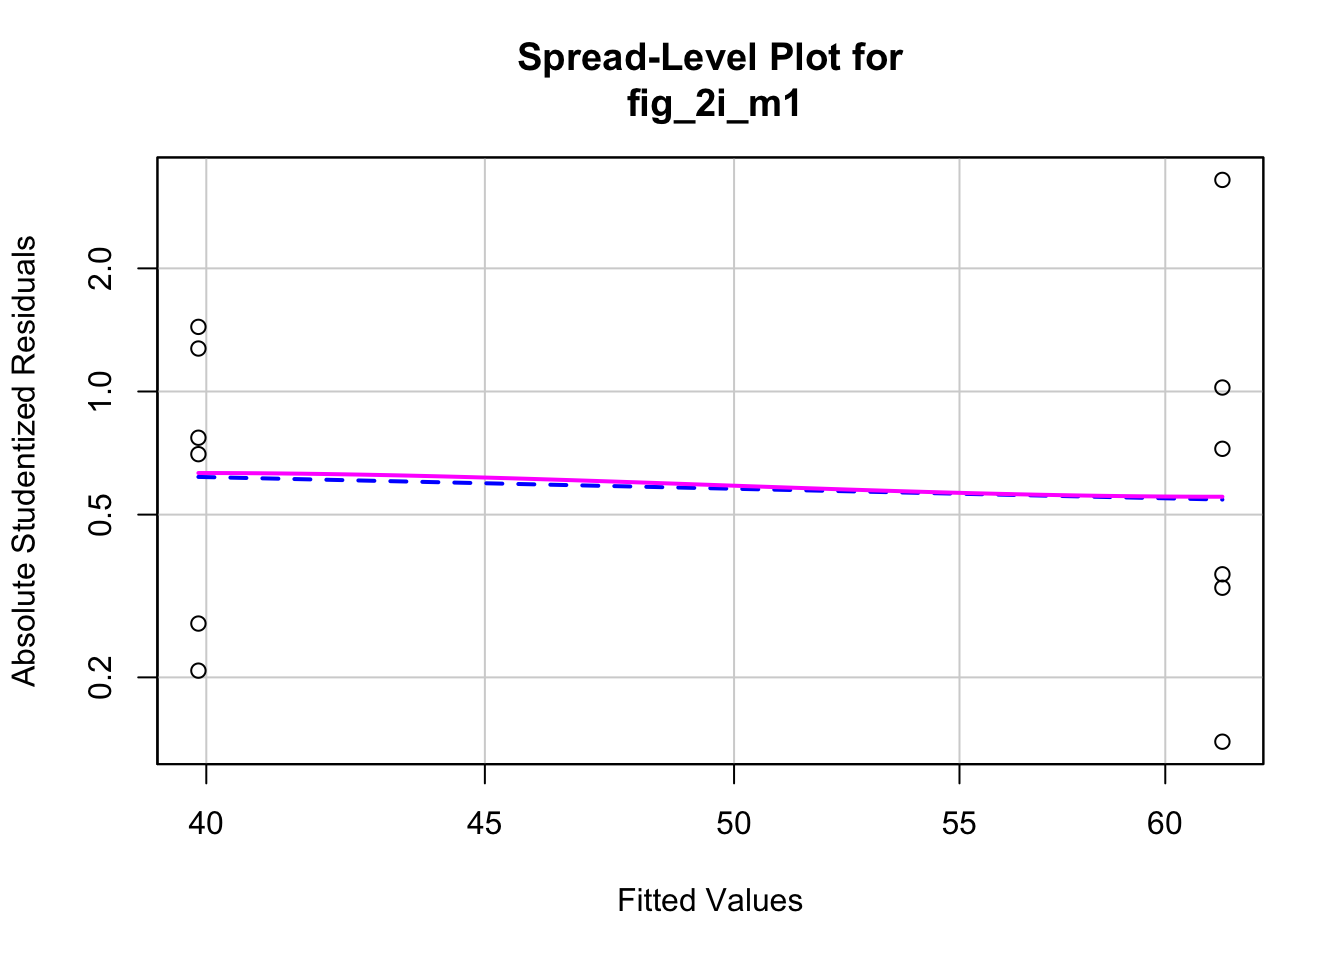
\includegraphics{Walker-elementary-statistical-odeling-draft_files/figure-latex/unnamed-chunk-5-1.pdf}

Compute the mean of the means

\begin{Shaded}
\begin{Highlighting}[]
\KeywordTok{mean}\NormalTok{(means)}
\end{Highlighting}
\end{Shaded}

\begin{verbatim}
## [1] -0.039961
\end{verbatim}

Questions

\begin{enumerate}
\def\labelenumi{\arabic{enumi}.}
\tightlist
\item
  Remember that the true mean is zero. How close, in general, are the
  sampled means to the true mean. How variable are the means? How is
  this quantified?
\item
  change n to 100, then replot. Are the means, in general, closer to the
  true mean? How variable are the means now?
\item
  Is the mean estimated with \(n=100\) closer to the truth, in general,
  then the mean estimated with \(n=6\)?
\item
  Redo with \(n=10000\)
\end{enumerate}

\subsection{part III - how do SD and SE change as sample size (n)
increases?}\label{part-iii---how-do-sd-and-se-change-as-sample-size-n-increases}

\begin{Shaded}
\begin{Highlighting}[]
\KeywordTok{mean}\NormalTok{(sds)}
\end{Highlighting}
\end{Shaded}

\begin{verbatim}
## [1] 1.017144
\end{verbatim}

Questions

\begin{enumerate}
\def\labelenumi{\arabic{enumi}.}
\tightlist
\item
  what is the mean of the standard deviations when n=6 (set p=1000)
\item
  what is the mean of the standard deviations when n=100 (set p=1000)
\item
  when n = 1000? (set p=1000)
\item
  when n = 10000? (set p=1000)
\item
  how does the mean of the standard deviations change as n increases
  (does it get smaller? or stay about the same size)
\item
  repeat the above with SEM
\end{enumerate}

\begin{Shaded}
\begin{Highlighting}[]
\KeywordTok{mean}\NormalTok{(sems)}
\end{Highlighting}
\end{Shaded}

\begin{verbatim}
## [1] 0.4152472
\end{verbatim}

Congratulations, you have just done a Monte Carlo simulation!

\subsection{\texorpdfstring{Part IV -- Generating fake data with ``for
loops''}{Part IV -- Generating fake data with for loops}}\label{part-iv-generating-fake-data-with-for-loops}

There are many other strategies for generating fake data -- two that
will be used extensively here are the funtion \texttt{rmvnorm()} and
\textbf{for loops}

\subsubsection{rmvnorm and a Covariance
Matrix}\label{rmvnorm-and-a-covariance-matrix}

We used the base R function \texttt{rnorm} above to generate
\texttt{fake\_data}, a matrix of random normal values. The columns are
generated independently of each other so the expected correlation
between any two columns is zero. The \texttt{rmvnorm()} (``random
multivariate normal'') function from the package \texttt{mvtnorm}
(``multivariate normal'') returns a matrix of random values drawn from a
multiviate normal distribution with a specified \textbf{covariance
matrix}. A covariance matrix is matrix of the variances and covariances
of the \(p\) columns of a data matrix. The \textbf{diagonal} of the
covariance matrix contains the variances of the \(p\) columns of the
data matrix and the off-diagonal elements contain the \(p(p-1)\)
pairwise covariances. The upper right set of covariances is the mirror
of the lower left set of covariates, so there are \(p(p-1)/2\) unique
covariances.

For our fake data, we want columns that are independent (E(COV) = 0) and
have expected variance of 1. This covariance matrix has a special name
-- the \textbf{identity matrix} (or sometimes ``unit'' matrix). Thus we
could use this script to generate fake data

\begin{Shaded}
\begin{Highlighting}[]
\NormalTok{n <-}\StringTok{ }\DecValTok{6} \CommentTok{# sample size}
\NormalTok{p <-}\StringTok{ }\DecValTok{10}\OperatorTok{^}\DecValTok{2} \CommentTok{# number of columns of fake data to generate}
\NormalTok{fake_data <-}\StringTok{  }\NormalTok{mvtnorm}\OperatorTok{::}\KeywordTok{rmvnorm}\NormalTok{(n, }\DataTypeTok{mean=}\KeywordTok{rep}\NormalTok{(}\DecValTok{0}\NormalTok{, p), }\DataTypeTok{sigma=}\KeywordTok{diag}\NormalTok{(p))}

\CommentTok{# compute the vectors of means, sds, and sems and the sd of the means}
\NormalTok{means <-}\StringTok{ }\KeywordTok{apply}\NormalTok{(fake_data,}\DecValTok{2}\NormalTok{,mean) }\CommentTok{# the apply function is super useful}
\NormalTok{sds <-}\StringTok{ }\KeywordTok{apply}\NormalTok{(fake_data,}\DecValTok{2}\NormalTok{,sd)}
\NormalTok{sems <-}\StringTok{ }\NormalTok{sds}\OperatorTok{/}\KeywordTok{sqrt}\NormalTok{(n)}
\KeywordTok{sd}\NormalTok{(means)}
\end{Highlighting}
\end{Shaded}

\begin{verbatim}
## [1] 0.4539342
\end{verbatim}

\begin{Shaded}
\begin{Highlighting}[]
\KeywordTok{mean}\NormalTok{(sems)}
\end{Highlighting}
\end{Shaded}

\begin{verbatim}
## [1] 0.4083748
\end{verbatim}

The vector of column means is specified using \texttt{mean=} and the
multivariate covariance matrix is specified with \texttt{sigma=} (the
lower case greek letter sigma (\(\sigma\)) is often used to denote a
population standard deviation. The upper case greek letter sigma
(\(\Sigma\)) is often used to denote a population covariance matrix).
This raises two questions

Questions.

\begin{enumerate}
\def\labelenumi{\arabic{enumi}.}
\tightlist
\item
  without using the console, what is returned with \texttt{rep(0,\ p)}?
\item
  without using the console, what is returned with \texttt{diag(p)}?
\item
  What are the \texttt{sd(means)} and \texttt{mean(sems)} comparing?
  What is the pedagogical purpose for adding this?
\end{enumerate}

Now use the console to check your answers.

\subsubsection{A for loop}\label{a-for-loop}

\begin{Shaded}
\begin{Highlighting}[]
\NormalTok{n <-}\StringTok{ }\DecValTok{6} \CommentTok{# sample size}
\NormalTok{n_iter <-}\StringTok{ }\DecValTok{10}\OperatorTok{^}\DecValTok{5} \CommentTok{# number of iterations of loop (equivalent to p)}
\NormalTok{means <-}\StringTok{ }\KeywordTok{numeric}\NormalTok{(n_iter)}
\NormalTok{sds <-}\StringTok{ }\KeywordTok{numeric}\NormalTok{(n_iter)}
\NormalTok{sems <-}\StringTok{ }\KeywordTok{numeric}\NormalTok{(n_iter)}
\ControlFlowTok{for}\NormalTok{(i }\ControlFlowTok{in} \DecValTok{1}\OperatorTok{:}\NormalTok{n_iter)\{}
\NormalTok{  y <-}\StringTok{ }\KeywordTok{rnorm}\NormalTok{(n) }\CommentTok{# mean=0 and sd=1 are default so not necessary to specify}
\NormalTok{  means[i] <-}\StringTok{ }\KeywordTok{mean}\NormalTok{(y)}
\NormalTok{  sds[i] <-}\StringTok{ }\KeywordTok{sd}\NormalTok{(y)}
\NormalTok{  sems[i] <-}\StringTok{ }\KeywordTok{sd}\NormalTok{(y)}\OperatorTok{/}\KeywordTok{sqrt}\NormalTok{(n)}
\NormalTok{\}}
\KeywordTok{sd}\NormalTok{(means)}
\end{Highlighting}
\end{Shaded}

\begin{verbatim}
## [1] 0.4090381
\end{verbatim}

\begin{Shaded}
\begin{Highlighting}[]
\KeywordTok{mean}\NormalTok{(sems)}
\end{Highlighting}
\end{Shaded}

\begin{verbatim}
## [1] 0.3883677
\end{verbatim}

Questions

\begin{enumerate}
\def\labelenumi{\arabic{enumi}.}
\tightlist
\item
  What do \texttt{sd(means)} and \texttt{mean(sems)} converge to as
  \texttt{n\_iter} is increased from 100 to 1000 to 10,000?
\item
  Do they converge to the same number?
\item
  Should they?
\item
  What is the correct number?
\end{enumerate}

Question number 4 is asking what is E(SEM), the ``expected standard
error of the mean''. There is a very easy formula to compute this. What
is it?

\chapter*{Appendix 1: Getting Started with
R}\label{appendix-1-getting-started-with-r}
\addcontentsline{toc}{chapter}{Appendix 1: Getting Started with R}

\section{Get your computer ready}\label{get-your-computer-ready}

\subsection{Install R}\label{install-r}

R is the core software

\href{https://cran.r-project.org}{Download R for your OS}

\subsection{Install R Studio}\label{install-r-studio}

R Studio is a slick (very slick) GUI interface for developing R projects

\href{https://www.rstudio.com/products/rstudio/download/}{Download R
Studio Desktop}

\subsection{Resources for installing R and R
Studio}\label{resources-for-installing-r-and-r-studio}

\href{https://medium.com/@GalarnykMichael/install-r-and-rstudio-on-windows-5f503f708027}{On
Windows}

\href{https://medium.com/@GalarnykMichael/install-r-and-rstudio-on-mac-e911606ce4f4}{On
a Mac}

\subsection{Install LaTeX}\label{install-latex}

LaTeX (``la-tek'') is necessary to use the pdf output of R Markdown.

\href{https://medium.com/@sorenlind/create-pdf-reports-using-r-r-markdown-latex-and-knitr-on-windows-10-952b0c48bfa9}{On
Windows}

\href{https://medium.com/@sorenlind/create-pdf-reports-using-r-r-markdown-latex-and-knitr-on-macos-high-sierra-e7b5705c9fd}{On
a Mac}

\section{Start learning}\label{start-learning}

\subsection{Start with Data Camp Introduction to
R}\label{start-with-data-camp-introduction-to-r}

\href{https://www.datacamp.com/courses/free-introduction-to-r}{Data
Camp: Introduction to R (free online course)}

\subsection{Then Move to Introduction to R
Studio}\label{then-move-to-introduction-to-r-studio}

\href{https://www.rstudio.com/resources/webinars/rstudio-essentials-webinar-series-part-1/}{R
Studio Essentials, Programming Part 1 (Writing code in RStudio)}

\subsection{Develop your project with an R Studio
Notebook}\label{develop-your-project-with-an-r-studio-notebook}

\href{https://www.rstudio.com/resources/webinars/getting-started-with-r-markdown/}{Getting
Started with R Markdown}

\href{https://www.rstudio.com/resources/webinars/introducing-notebooks-with-r-markdown/}{Introducing
Notebooks with R Markdown}

\section{Getting Data into R}\label{getting-data-into-r}

\href{https://www.rstudio.com/resources/webinars/getting-your-data-into-r/}{Getting
your data into R}

\section{Additional R learning
resources}\label{additional-r-learning-resources}

\href{https://bookdown.org/chesterismay/rbasics/}{Getting used to R,
RStudio, and R Markdown}

\href{https://www.rstudio.com/resources/webinars/}{Link to list of R
Studio webinars}

\href{https://www.rstudio.com/resources/cheatsheets/}{Link to set of R
package cheat sheets (amazing!)}

\href{https://bookdown.org}{Bookdown online books}

\section{Packages used extensively in this
text}\label{packages-used-extensively-in-this-text}

\begin{enumerate}
\def\labelenumi{\arabic{enumi}.}
\tightlist
\item
  ggplot2
\item
  data.table
\item
  mvtnorm
\item
  lme4
\item
  nlme
\item
  emmeans
\item
  readxl
\item
  reshape2
\end{enumerate}

\href{http://r4ds.had.co.nz/data-visualisation.html}{Data Visualisation
chapter from \emph{R for Data Science}}

\href{http://r4ds.had.co.nz/graphics-for-communication.html}{Graphics
for communication chapter from \emph{R for Data Science}}

Youtube: \href{https://www.youtube.com/watch?v=pc1ARG6kbAM}{An
Introduction to The data.table Package}

Coursera:
\href{https://www.coursera.org/learn/data-cleaning/lecture/trMZ7/the-data-table-package}{The
data.table Package}

\chapter*{Appendix 2: Online Resources for Getting Started with Linear
Modeling in
R}\label{appendix-2-online-resources-for-getting-started-with-linear-modeling-in-r}
\addcontentsline{toc}{chapter}{Appendix 2: Online Resources for Getting
Started with Linear Modeling in R}

\href{https://leanpub.com/regmods}{Regression Models for Data Science in
R by Brian Caffo}

\href{https://bookdown.org/roback/bookdown-bysh/}{Broadening Your
Statistical Horizons: Generalized Linear Models and Multilevel Models by
J. Legler and P. Roback}

\href{https://bookdown.org/rdpeng/artofdatascience/}{The Art of Data
Science by Roger D. Peng and Elizabeth Matsui}

\bibliography{book.bib,packages.bib}


\end{document}
